% Welcome! This is the unofficial University of Udine beamer template.

% See README.md for more informations about this template.

% This style has been developed following the "Manuale di Stile"
% (Style Manual) of the University of Udine. You can find the
% manual here: https://www.uniud.it/it/ateneo-uniud/ateneo-uniud/identita-visiva/manuali-immagine-stile/manuale-stile

% Note: for some reason, the RGB values specified in the manual
% do NOT render correctly in Beamer, so they have been redefined
% for this document using the high level chromo-optic deep neural
% quantistic technology offered by Microsoft Paint's color picker.

% We defined four theme colors: UniBrown, UniBlue, UniGold
% and UniOrange. For example, to write some uniud-brownish
% text, just use: \textcolor{UniBrown}{Hello!}

% Note that [usenames,dvipsnames] is MANDATORY due to compatibility
% issues between tikz and xcolor packages.

\documentclass[usenames,dvipsnames]{beamer}
\usepackage[utf8]{inputenc}
\usepackage{verbatim}
\usetheme{uniud}

% cleverref {{{
\usepackage[capitalize,nameinlink]{cleveref} % from https://tex.stackexchange.com/questions/187388/amsthm-with-shared-counters-messes-up-autoref-references
% }}}

\usepackage{graphicx}

%%% Bibliography {{{
\usepackage[style=authoryear,backend=biber]{biblatex}
\addbibresource{bibliography.bib}

% Author names in publication list are consistent
% i.e. name1 surname1, name2 surname2
% See https://tex.stackexchange.com/questions/106914/biblatex-does-not-reverse-the-first-and-last-names-of-the-second-author
\DeclareNameAlias{author}{first-last}
% }}}

%%% Suppress biblatex annoying warning {{{
\usepackage{silence}
\WarningFilter{biblatex}{Patching footnotes failed}
% }}}

%%% Some useful commands {{{
% pdf-friendly newline in links
\newcommand{\pdfnewline}{\texorpdfstring{\newline}{ }}
% Fill the vertical space in a slide (to put text at the bottom)
\newcommand{\framefill}{\vskip0pt plus 1filll}
% }}}


% \title[University of Udine Unofficial Beamer Theme]{Report: A formal approach for run-time verification of web applications using scope-extended LTL}
\title{Run-time verification of web applications}
% \date[May 1977]{May 25, 1977}
\author[Roberto Tonino]{
  Roberto Tonino
  \pdfnewline
  \texttt{tonino.roberto@spes.uniud.it}
}
\institute{\tiny Department of Mathematics, Computer Science and Physics, University of Udine}

% glossary {{{
\usepackage[acronym,automake]{glossaries}
\makeglossaries

% \newglossaryentry{WAUT}
% {
%     name=WAUT,
%     description={Web Application Under Test}
% }
\newacronym{waut}{WAUT}{Web Application Under Test}
% }}}


\begin{document}

\begin{frame}
\titlepage
\end{frame}

\begin{frame}{Outline}
\tableofcontents
\end{frame}

% \section{Before you start}
% \begin{frame}{Overleaf users}

% \begin{alertblock}{Warning}
% You can ignore this slide if you're \textbf{not} working with Overleaf.
% \end{alertblock}

% \vskip 0.5cm

% Overleaf, Beamer and Biber do not always get along well together. For this reason, if you make a mistake while writing this presentation, in the drop-down error message you'll \textbf{always} get Biber-related error messages.

% \vskip 0.5cm

% Luckily, you just have to click on ``\texttt{go to first error/warning}'' and the UI will scroll to the line containing your mistake.

% \end{frame}

\section{Introduction}
\begin{frame}{Introduction}

This report summarizes the paper \citetitle{Haydar2013}.
\end{frame}

\framecard{Automata}

\section{Automata}
\begin{frame}{Automata}

  The authors of the paper propose an automata-based model of the \gls{waut}. It is important to note that this model is \textbf{not exaustive}; it is instead to be considered an extension of traditional testing. The authors consider two settings---single-window applications and multi-window applications---with which they build the model solution in two phases. The single-window application model is first proposed in order to then be enhanced by the multi-window application model.

\end{frame}

\subsection{Single-window applications}
\begin{frame}{Single-window applications}
\label{single-window-applications}

The automata from a single-window application is built as follows:

\begin{enumerate}
  \item the inactive state is defined;
  \item the set of states is defined by the set of responses, except when only the links in the responses are different, in which case the responses are mapped to the same state;
  \item the alphabet is built from the union of the links, the requests and the unexplored forms;
  \item the transitions are defined by one state to another if there is a link or a form action that takes from one page to another;
  \item ?
  \item for each unexplored link or form, the automaton has a transition to a so-called ``trap'' state.
\end{enumerate}

\end{frame}

\begin{frame}{Single-window applications}

The construction allows to define \emph{deduced} links: they are links that are not visited during the browsing session, but are contained in one or more of the responses of the browsing session. Deduced links extend the automaton, making it slightly more complete and improving reachability.

In \cref{fig:example-session-automaton} it is possible to see an example of a constructed session automaton.

\begin{figure}[h]
  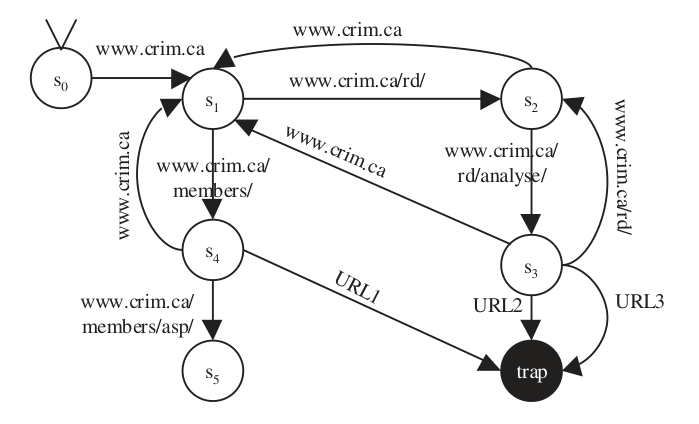
\includegraphics[width=\textwidth]{../img/session_automaton_example.png}
  \caption{Example of a session automaton.}
  \label{fig:example-session-automaton}
\end{figure}

\end{frame}

\subsection{Multi-window applications}

\begin{frame}{Multi-window applications}

The model presented in \cref{single-window-applications} is extended to handle multi-window applications.

\begin{itemize}
  \item the elements in the set of links are extended with the link target
  \item the elements in the set of form actions are extended with the link target
  \item the requests are now made of the link as before, with the addition of the referer (link from which the request started) and the target
\end{itemize}

\end{frame}

\begin{frame}{Multi-window applications}
The procedure for single-window applications is extended as follows:

\begin{enumerate}
  \item a browsing session is split in local browsing sessions---one for each window and frame;
  \item convert every local browsing session into an automaton;
  \item the alphabet of the final automaton is extended with the source pages of the frames (src attribute);
  \item the case in which the user clicks on a link or submits a form while a frame is loading is handled by adding a transition from each state of the local automaton to the response state.
\end{enumerate}

This is called ``communicating automata model'' and is explained in detail in \cite{Haydar2004}.

\end{frame}

\section{LTL}
\begin{frame}{LTL}

To ease the definition of properties in web applications, the authors introduce a syntax sugar to increase succintness of LTL. The syntax sugar allows one to specify LTL properties over a subset of propositions. In the web setting, this can be used to, e.g., specify properties that hold only on the main page, or only in a subset of the pages of the application.

Over logical properties, the $\mathcal{\Im}$-scope operator is introduced. The authors re-define LTL's $\neg$, $\land$, U, X, F, and G operators. Over logical formulas, the \textbf{\texttt{In}} operator is introduced, which makes use of the $\mathcal{\Im}$-scope operator. The full specification is detailed in \cite{Haydar2005}.

\end{frame}

\section{Evaluation of the results}
\begin{frame}{Evaluation of the results}

\subsection{Theoretical evaluation}

The authors propose a theoretical evaluation that assume that all pages are static, i.e. there are no scripts running in them, the \gls{waut} is static, i.e. during the observation it doesn't variate, that there is a one-to-one mapping between an URI and a page, and that always $c = 200$.

The definition of a (finite) web app automaton is then given. The authors then present a theorem that states that each trace of a session automaton is also a trace of a web app automaton.

After this, a generalization to Kripke structures is made. The definition of a Kripke structure of a web application and of a browsing session are given. Then, a theorem that states that the browsing session Kripke structure is a ``reduced abstraction'' of a web app Kripke structure. This means that if a property is violated in the browsing session Kripke structure, then it is also violated in the web application Kripke structure, for infinite counterexamples. For finite counterexamples, only \textit{safety} properties keep this claim.

\end{frame}

\subsection{Implementation and empirical evaluation}
\begin{frame}{Implementation and empirical evaluation}

The authors built a tool that can record a browsing session, build an internal representation of the session, evaluate a set of properties against the internal representation, and visualize the automata. The set of properties can be split into general properties---applicable to every web app in existence---also defined as non-functional, and specific properties also defined as functional.

The exploration was performed on a number of websites chosen by the authors. Part of the websites were explored manually (by a human), and part by a crawler. The crawler performed a \emph{complete} exploration: all the pages of the web app were explored.

Many of the defined properties were violated. The authors note how small and large web applications have a lower number of violations, while medium-sized applications have the highest.

(Example of a property + counterexample)

(Example of a \textit{valid} negation of a property)

\end{frame}

\section{Conclusions}

\begin{frame}{Conclusions}

It is important to notice how the rapid change of web development has impacted the results of this paper. The frames approach is not common anymore (even though micro-frontends are on the rise (TODO cite)), but the biggest change is that server-rendered HTML is not the standard in web applications anymore (while in websites, the situation differs).

\end{frame}

\end{document}

% vi: fdm=marker
